\begin{frame}{Contributions}\framesubtitle{TopicCoRank}
  Adaptation supervisée de TopicRank aux domaines de spécialité

  \vspace{1em}

  \begin{block}{Objectif}
    Réaliser conjointement extraction et assignement
  \end{block}

  \vspace{1em}

  \begin{block}{Hypothèse}
    Les documents d'apprentissage se suffisent au domaine~:
    \begin{itemize}
      \item{Termes-clés $\simeq$ vocabulaire du domaine}
      \item{Cohérence entre les termes-clés d'un même document}
    \end{itemize}
  \end{block}
\end{frame}

\begin{frame}{TopicCoRank}\framesubtitle{Aperçu}
  Méthode en 8 étapes~:
  \begin{enumerate}
    \item{Déduction du vocabulaire contrôlé du domaine}
    \item{Création du graphe des termes-clés du domaine}
    \vspace{.75em}\hrule\vspace{.5em}
    \item{Sélection des termes-clés candidats du document}
    \item{Groupement des candidats en sujets}
    \item{Création du graphe de sujets}
    \vspace{.75em}\hrule\vspace{.5em}
    \item{Unification du graphe de sujets au graphe du domaine}
    \item{Ordonnancement conjoint des sujets et des termes-clés du domaine}
    \item{Sélection des termes-clés parmi les meilleurs sujets et/ou termes-clés
          du domaine}
  \end{enumerate}
\end{frame}

\begin{frame}{TopicCoRank}\framesubtitle{Exemple}
  \vspace{-.33em}
  \begin{exampleblock}{\small
    Étude préliminaire de la céramique non tournée micacée du bas Languedoc
    occidental~: typologie, chronologie et aire de diffusion
  }\justifying\small
    ~~~L'étude présente une variété de céramique non tournée dont la typologie
    et l'analyse des décors permettent de l'identifier facilement. La nature de
    l'argile enrichie de mica donne un aspect pailleté à la pâte sur laquelle le
    décor effectué selon la méthode du brunissoir apparaît en traits brillant
    sur fond mat. Cette première approche se fonde sur deux séries issues de
    fouilles anciennes menées sur les oppidums du Cayla à Mailhac (Aude) et de
    Mourrel-Ferrat à Olonzac (Hérault). La carte de répartition fait état
    d'échanges ou de commerce à l'échelon macrorégional rarement mis en évidence
    pour de la céramique non tournée. S'il est difficile de statuer sur
    l'origine des décors, il semble que la production s'insère dans une ambiance
    celtisante. La chronologie de cette production se situe dans le deuxième âge
    du Fer. La fourchette proposée entre la fin du IV$^\text{e}$ et la fin du
    II$^\text{e}$ s. av. J.-C. reste encore à préciser.

    \begin{exampleblock}{\small Termes-clés}\justifying\small
      \underline{Mailhac}~; \underline{Aude}~; \underline{Mourrel-Ferrat}~;
      \underline{Olonzac}~; \underline{Hérault}~; \underline{céramique}~;
      \underline{typologie}~; \underline{décor}~; \underline{chronologie}~;
      \underline{diffusion}~; \underline{production}~; \underline{commerce}~;
      \underline{répartition}~; \underline{oppidum}~; \underline{analyse}~;
      \underline{fouille ancienne}~; Europe~; France~; le Cayla~; La Tène~;
      celtes~; distribution~; micassé~; céramique non-tournée~; echange~;
      cartographie~; habitat~; site fortifié~; identification~; étude du
      matériel~; age du fer.
    \end{exampleblock}
  \end{exampleblock}
\end{frame}

\begin{frame}{TopicCoRank}\framesubtitle{Exemple}
  \newcommand{\xslant}{0.25}
  \newcommand{\yslant}{0}
  \centering
  \begin{tikzpicture}[transform shape, scale=.75]
    % frames %%%%%%%%%%%%%%%%%%%%%%%%%%%%%%%%%%%%%%%%%%%%%%%%%%%%%%%%%%%%%%%%%%%
    \uncover<3->{
      \node [draw,
             rectangle,
             minimum width=1.15\linewidth,
             minimum height=.5\textheight,
             xslant=\xslant,
             yslant=\yslant] (domain_graph) {};
    }
    \node [draw,
          rectangle,
          minimum width=1.15\linewidth,
          minimum height=.5\textheight,
          xslant=\xslant,
          yslant=\yslant,
          above=of domain_graph,
          xshift=-3.5em] (document_graph) {};

    % domain %%%%%%%%%%%%%%%%%%%%%%%%%%%%%%%%%%%%%%%%%%%%%%%%%%%%%%%%%%%%%%%%%%%
    \node [above=of domain_graph,
           xshift=.575\linewidth,
           yshift=.5\textheight,
           anchor=south east] (domain_graph_label) {termes-clés du domaine (sous-partie)};

    % nodes
    \node [above=of domain_graph,%draw,
           xshift=-1.9em,
           yshift=.425\textheight] (france) {\alt<6->{\textcolor{termithorange}{\textbf{France}}}{France}};
    \node [above=of domain_graph,%draw,
           xshift=-7.5em,
           yshift=.29\textheight] (typologie) {typologie};
    \node [above=of domain_graph,%draw,
           xshift=4.3em,
           yshift=.29\textheight] (chronologie) {chronologie};
    \node [above=of domain_graph,%draw,
           xshift=-16.5em,
           yshift=.22\textheight] (ceramique) {céramique};
    \node [above=of domain_graph,%draw,
           xshift=13em,
           yshift=.22\textheight] (production) {production};
    \node [above=of domain_graph,%draw,
           xshift=2.2em,
           yshift=.1\textheight] (analyse) {\alt<6->{\textcolor{termithorange}{\textbf{analyse}}}{analyse}};
    \node [above=of domain_graph,%draw,
           xshift=-5.2em,
           yshift=.1\textheight] (decor) {décor};
    \node [above=of domain_graph,%draw,
           xshift=-12.5em,
           yshift=.01\textheight] (repartition) {répartition};
    \node [above=of domain_graph,%draw,
           xshift=9.5em,
           yshift=.02\textheight] (diffusion) {diffusion};

    \uncover<2->{
      % france
      \draw (france) -- (typologie);
      \draw (france) -- (chronologie);
      \draw (france) -- (production);
      \draw (france) -- (diffusion);
      \draw (france) -- (decor);
      \draw (france) -- (analyse);
      \draw (france) -- (repartition);
      \draw (france) -- (ceramique);
      % typologie
      \draw (typologie) -- (chronologie);
      \draw (typologie) -- (production);
      \draw (typologie) -- (diffusion);
      \draw (typologie) -- (decor);
      \draw (typologie) -- (analyse);
      \draw (typologie) -- (repartition);
      \draw (typologie) -- (ceramique);
      % chronologie
      \draw (chronologie) -- (production);
      \draw (chronologie) -- (diffusion);
      \draw (chronologie) -- (decor);
      \draw (chronologie) -- (analyse);
      \draw (chronologie) -- (repartition);
      \draw (chronologie) -- (ceramique);
      % production
      \draw (production) -- (diffusion);
      \draw (production) -- (decor);
      \draw (production) -- (analyse);
      \draw (production) -- (ceramique);
      % diffusion
      \draw (diffusion) -- (decor);
      \draw (diffusion) -- (analyse);
      \draw (diffusion) -- (ceramique);
      % decor
      \draw (decor) -- (analyse);
      \draw (decor) -- (ceramique);
      % analyse
      \draw (analyse) -- (ceramique);
    }

    % document %%%%%%%%%%%%%%%%%%%%%%%%%%%%%%%%%%%%%%%%%%%%%%%%%%%%%%%%%%%%%%%%%
    \uncover<3->{
      \node [below=of document_graph,
             xshift=-.575\linewidth,
             yshift=-.5\textheight,
             anchor=north west] (document_graph_label) {sujets du document (sous-partie)};

      \node [minimum width=2.5em,
             below=of document_graph,%draw,
             xshift=-4em,
             yshift=-.05\textheight] (typologie_c) {\alt<6->{\textcolor{termithorange}{\textbf{[typologie]}}}{[typologie]}};
      \node [minimum width=2.5em,
             below=of document_graph,%draw,
             xshift=10.75em,
             yshift=-.05\textheight] (chronologie_c) {\alt<6->{\textcolor{termithorange}{\textbf{[chronologie]}}}{[chronologie]}};
      \node [minimum width=2.5em,
             below=of document_graph,%draw,
             xshift=-13.1em,
           yshift=-.25\textheight] (ceramique_c) {\alt<6->{\textcolor{termithorange}{\textbf{[céramique]}}}{[céramique]}};
      \node [minimum width=2.5em,
             below=of document_graph,%draw,
             xshift=17em,
             yshift=-.125\textheight] (production_c) {\alt<6->{\textcolor{termithorange}{\textbf{[production]}}}{[production]}};
      \node [minimum width=2.5em,
             below=of document_graph,%draw,
             xshift=2.5em,
             yshift=-.25\textheight] (analyse_c) {[analyse]};
      \node [minimum width=2.5em,
             below=of document_graph,%draw,
             xshift=.5em,
             yshift=-.40\textheight] (decor_c) {\alt<6->{\textcolor{termithorange}{\textbf{[décors~; décor]}}}{[décors~; décor]}};
      \node [minimum width=2.5em,
             below=of document_graph,%draw,
             xshift=-9em,
             yshift=-.40\textheight] (repartition_c) {\alt<6->{\textcolor{termithorange}{\textbf{[répartition]}}}{[répartition]}};
      \node [minimum width=2.5em,
             below=of document_graph,%draw,
             xshift=15em,
             yshift=-.40\textheight] (diffusion_c) {\alt<6->{\textcolor{termithorange}{\textbf{[diffusion]}}}{[diffusion]}};
      \node [minimum width=2.5em,
             below=of document_graph,%draw,
             xshift=7.66em,
             yshift=-.16\textheight] (etude_preliminaire_c) {\alt<6->{\textcolor{termithorange}{\textbf{[étude préliminaire]}}}{[étude préliminaire]}};
      \node [minimum width=2.5em,
             below=of document_graph,%draw,
             xshift=17em,
             yshift=-.25\textheight] (fer_c) {[fer]};
    }

    \uncover<4->{
      % typologie
      \draw (typologie_c) -- (chronologie_c);
      \draw (typologie_c) -- (diffusion_c);
      \draw (typologie_c) -- (decor_c);
      \draw (typologie_c) -- (analyse_c);
      \draw (typologie_c) -- (ceramique_c);
      % chronologie
      \draw (chronologie_c) -- (production_c);
      \draw (chronologie_c) -- (diffusion_c);
      \draw (chronologie_c) -- (ceramique_c);
      % production
      \draw (production_c) -- (decor_c);
      % diffusion
      \draw (diffusion_c) -- (ceramique_c);
      % decor
      \draw (decor_c) -- (analyse_c);
      \draw (decor_c) -- (repartition_c);
      \draw (decor_c) -- (ceramique_c);
      % analyse
      \draw (analyse_c) -- (ceramique_c);
      % répartition
      \draw (repartition_c) -- (ceramique_c);
      % étude préliminaire
      \draw (etude_preliminaire_c) -- (ceramique_c);
      \draw (etude_preliminaire_c) -- (chronologie_c);
      \draw (etude_preliminaire_c) -- (typologie_c);
      \draw (etude_preliminaire_c) -- (diffusion_c);
      % fer
      \draw (fer_c) -- (chronologie_c);
      \draw (fer_c) -- (production_c);
    }

    % extra link %%%%%%%%%%%%%%%%%%%%%%%%%%%%%%%%%%%%%%%%%%%%%%%%%%%%%%%%%%%%%%%
    \uncover<5->{
      \draw [dashed] (typologie) -- (typologie_c);
      \draw [dashed] (chronologie) -- (chronologie_c);
      \draw [dashed] (ceramique) -- (ceramique_c);
      \draw [dashed] (production) -- (production_c);
      \draw [dashed] (analyse) -- (analyse_c);
      \draw [dashed] (decor) -- (decor_c);
      \draw [dashed] (repartition) -- (repartition_c);
      \draw [dashed] (diffusion) -- (diffusion_c);
    }
  \end{tikzpicture}
\end{frame}

\begin{frame}{TopicCoRank}\framesubtitle{Exemple}
  \begin{table}
      \centering
      \begin{tabular}{r|l|l}
        \toprule
        \textbf{Rang} & \multicolumn{1}{c|}{\textbf{TopicRank}} & \multicolumn{1}{c}{\textbf{TopicCoRank}} \\
        \hline
        01 & \cellcolor{termithorange!30}{décors} & \cellcolor{termithorange!30}{céramique} \\
        02 & \cellcolor{termithorange!30}{céramique} & \cellcolor{termithorange!30}{décors} \\
        03 & \cellcolor{termithorange!30}{chronologie} & \cellcolor{termithorange!30}{typologie} \\
        04 & \cellcolor{termithorange!30}{typologie} & \cellcolor{termithorange!30}{chronologie} \\
        05 & \cellcolor{termithorange!30}{production} & \cellcolor{termithorange!30}{production} \\
        06 & fin & étude préliminaire \\
        07 & étude préliminaire & \cellcolor{termithorange!30}{diffusion} \\
        08 & fer & \cellcolor{Cerulean!30}{analyse} \\
        09 & deuxième âge & \cellcolor{Cerulean!30}{France} \\
        10 & aire & \cellcolor{termithorange!30}{répartition} \\
        \bottomrule
      \end{tabular}

      \caption{Termes-clés}
    \end{table}

    \begin{block}{Observations}
      \begin{itemize}
        \item{Amélioration de l'ordonnancement grâce au domaine}
        \item{Assignement de \og{}France\fg{} (hors document)}
      \end{itemize}
    \end{block}
\end{frame}

\begin{frame}{TopicCoRank}\framesubtitle{Évaluation}
  \begin{columns}
    \begin{column}{.6\textwidth}
      Trois méthodes de référence~:
      \begin{itemize}
        \item{TF-IDF~\cite{salton1975tfidf}}
        \item{TopicRank~\cite{bougouin2013topicrank}}
        \item{KEA++~\cite{medelyan2006kea++}}
      \end{itemize}

      \vspace{1em}

      Deux variantes~:
      \begin{itemize}
        \item{TopicCoRank$_\text{extr.}$}
        \item{TopicCoRank$_\text{assign.}$}
      \end{itemize}

      \vspace{1em}

      Évaluation à 10 termes-clés, en termes de~:
      \begin{itemize}
        \item{Précision (P)~: $\frac{|\text{corrects}|}{|\text{extraits}|}$}
        \item{Rappel (R)~: $\frac{|\text{corrects}|}{|\text{references}|}$}
        \item{F1-mesure (F)~: $2 \times \frac{\text{précision} \times \text{rappel}}{\text{précision} + \text{rappel}}$}
      \end{itemize}
    \end{column}

    \begin{column}{.4\textwidth}
      \centering
      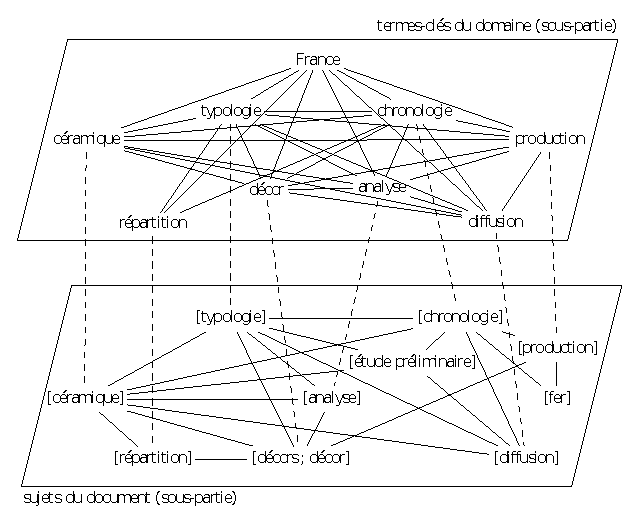
\includegraphics[width=.8\textwidth]{include/topiccorank_graph.eps}
    \end{column}
  \end{columns}
\end{frame}

\begin{frame}{TopicCoRank}\framesubtitle{Résultats}
  \begin{table}
    \resizebox{\linewidth}{!}{
      \begin{tabular}{@{~}l|c@{~~}c@{~~}c@{~}|c@{~~~~~~~~}c@{~~~~~~}c@{~}|c@{~~}c@{~~}c@{~}|c@{~~}c@{~~}c@{~}}
        \toprule
        \multirow{2}{*}{\textbf{Méthode}} & \multicolumn{3}{c|}{\textbf{Linguistique} \textit{(fr)}} & \multicolumn{3}{c|}{\textbf{Sciences de l'info.} \textit{(fr)}} & \multicolumn{3}{c|}{\textbf{Archéologie} \textit{(fr)}} & \multicolumn{3}{c}{\textbf{Chimie} \textit{(fr)}}\\
        \cline{2-13}
        & P & R & F & P & R & F & P & R & F & P & R & F\\
        \hline
        \textsc{Tf-Idf} & 13,0 & 15,4 & 13,9 & 13,4 & 14,0 & 13,2$^{~}$ & 28,1 & 19,1 & 22,2$^{~~}$ & 14,1 & 11,1 & 11,9$^{~~}$\\
        TopicRank & 11,2 & 13,1 & 11,9 & 12,1 & 12,8 & 12,1$^{~}$ & 27,5 & 18,7 & 21,8$^{~~}$ & 13,8 & 11,1 & 11,8$^{~~}$\\
        KEA++ & 11,6 & 13,0 & 12,1 & $~~$9,5 & 10,2 & $~~$9,6$^{~~}$ & 23,5 & 16,2 & 18,8$^{~~}$ & 11,4 & $~~$8,5 & $~~$9,2$^{~~}$\\
        \hline
        TopicCoRank$_\textnormal{extr.}$ & 14,3 & 16,5 & 15,1 & 15,4 & 15,9 & 15,2$^\dagger$ & 36,7 & 24,6 & 28,8$^\dagger$ & 15,8 & 12,1 & 13,1$^{~~}$\\
        TopicCoRank$_\textnormal{assign.}$ & \textbf{24,5} & \textbf{28,3} & \textbf{25,8} & \textbf{19,7} & \textbf{19,8} & \textbf{19,2}$^\dagger$ & \textbf{47,8} & \textbf{32,3} & \textbf{37,7}$^\dagger$ & \textbf{20,0} & \textbf{14,8} & \textbf{16,3}$^\dagger$\\
        \hline
        TopicCoRank & 18,8 & 21,9 & 19,9 & 17,3 & 17,7 & 17,0$^\dagger$ & 38,3 & 25,7 & 30,1$^\dagger$ & 17,2 & 13,4 & 14,4$^\dagger$\\
        \bottomrule
      \end{tabular}
    }
  \end{table}

  \vspace{1em}

  \begin{block}{Observations}
    \begin{itemize}
      \item{Meilleure performance}
      \item{TopicCoRank$_\text{assign.}$ $>$ TopicCoRank $>$
            TopicCoRank$_\text{extr.}$}
      \item{TopicCoRank$_\text{extr.}$ $>$ TopicRank $\Rightarrow$ apport du
            domaine}
    \end{itemize}
  \end{block}
\end{frame}

\begin{frame}{TopicCoRank}\framesubtitle{Bilan}
  Méthode supervisée à base de graphe qui tire profit du domaine de spécialité
  pour améliorer l'ordonnancement des sujets de TopicRank et permettre
  l'assignement de termes-clés

  \vspace{1em}

  \begin{block}{Avantages}
    \begin{itemize}
      \item{Exploite les données d'entraînement plus finement}
      \item{Couvre tous les besoins}
    \end{itemize}
  \end{block}

  \vspace{1em}

  \begin{alertblock}{Limites}
    \begin{itemize}
      \item{Donne autant d'importance aux deux graphes}
      \item{Plus redondant que TopicRank}
    \end{itemize}
  \end{alertblock}
\end{frame}

